% \documentclass{article}
\documentclass[tikz,margin=5mm]{standalone}
\usepackage{tikz}
\begin{document}
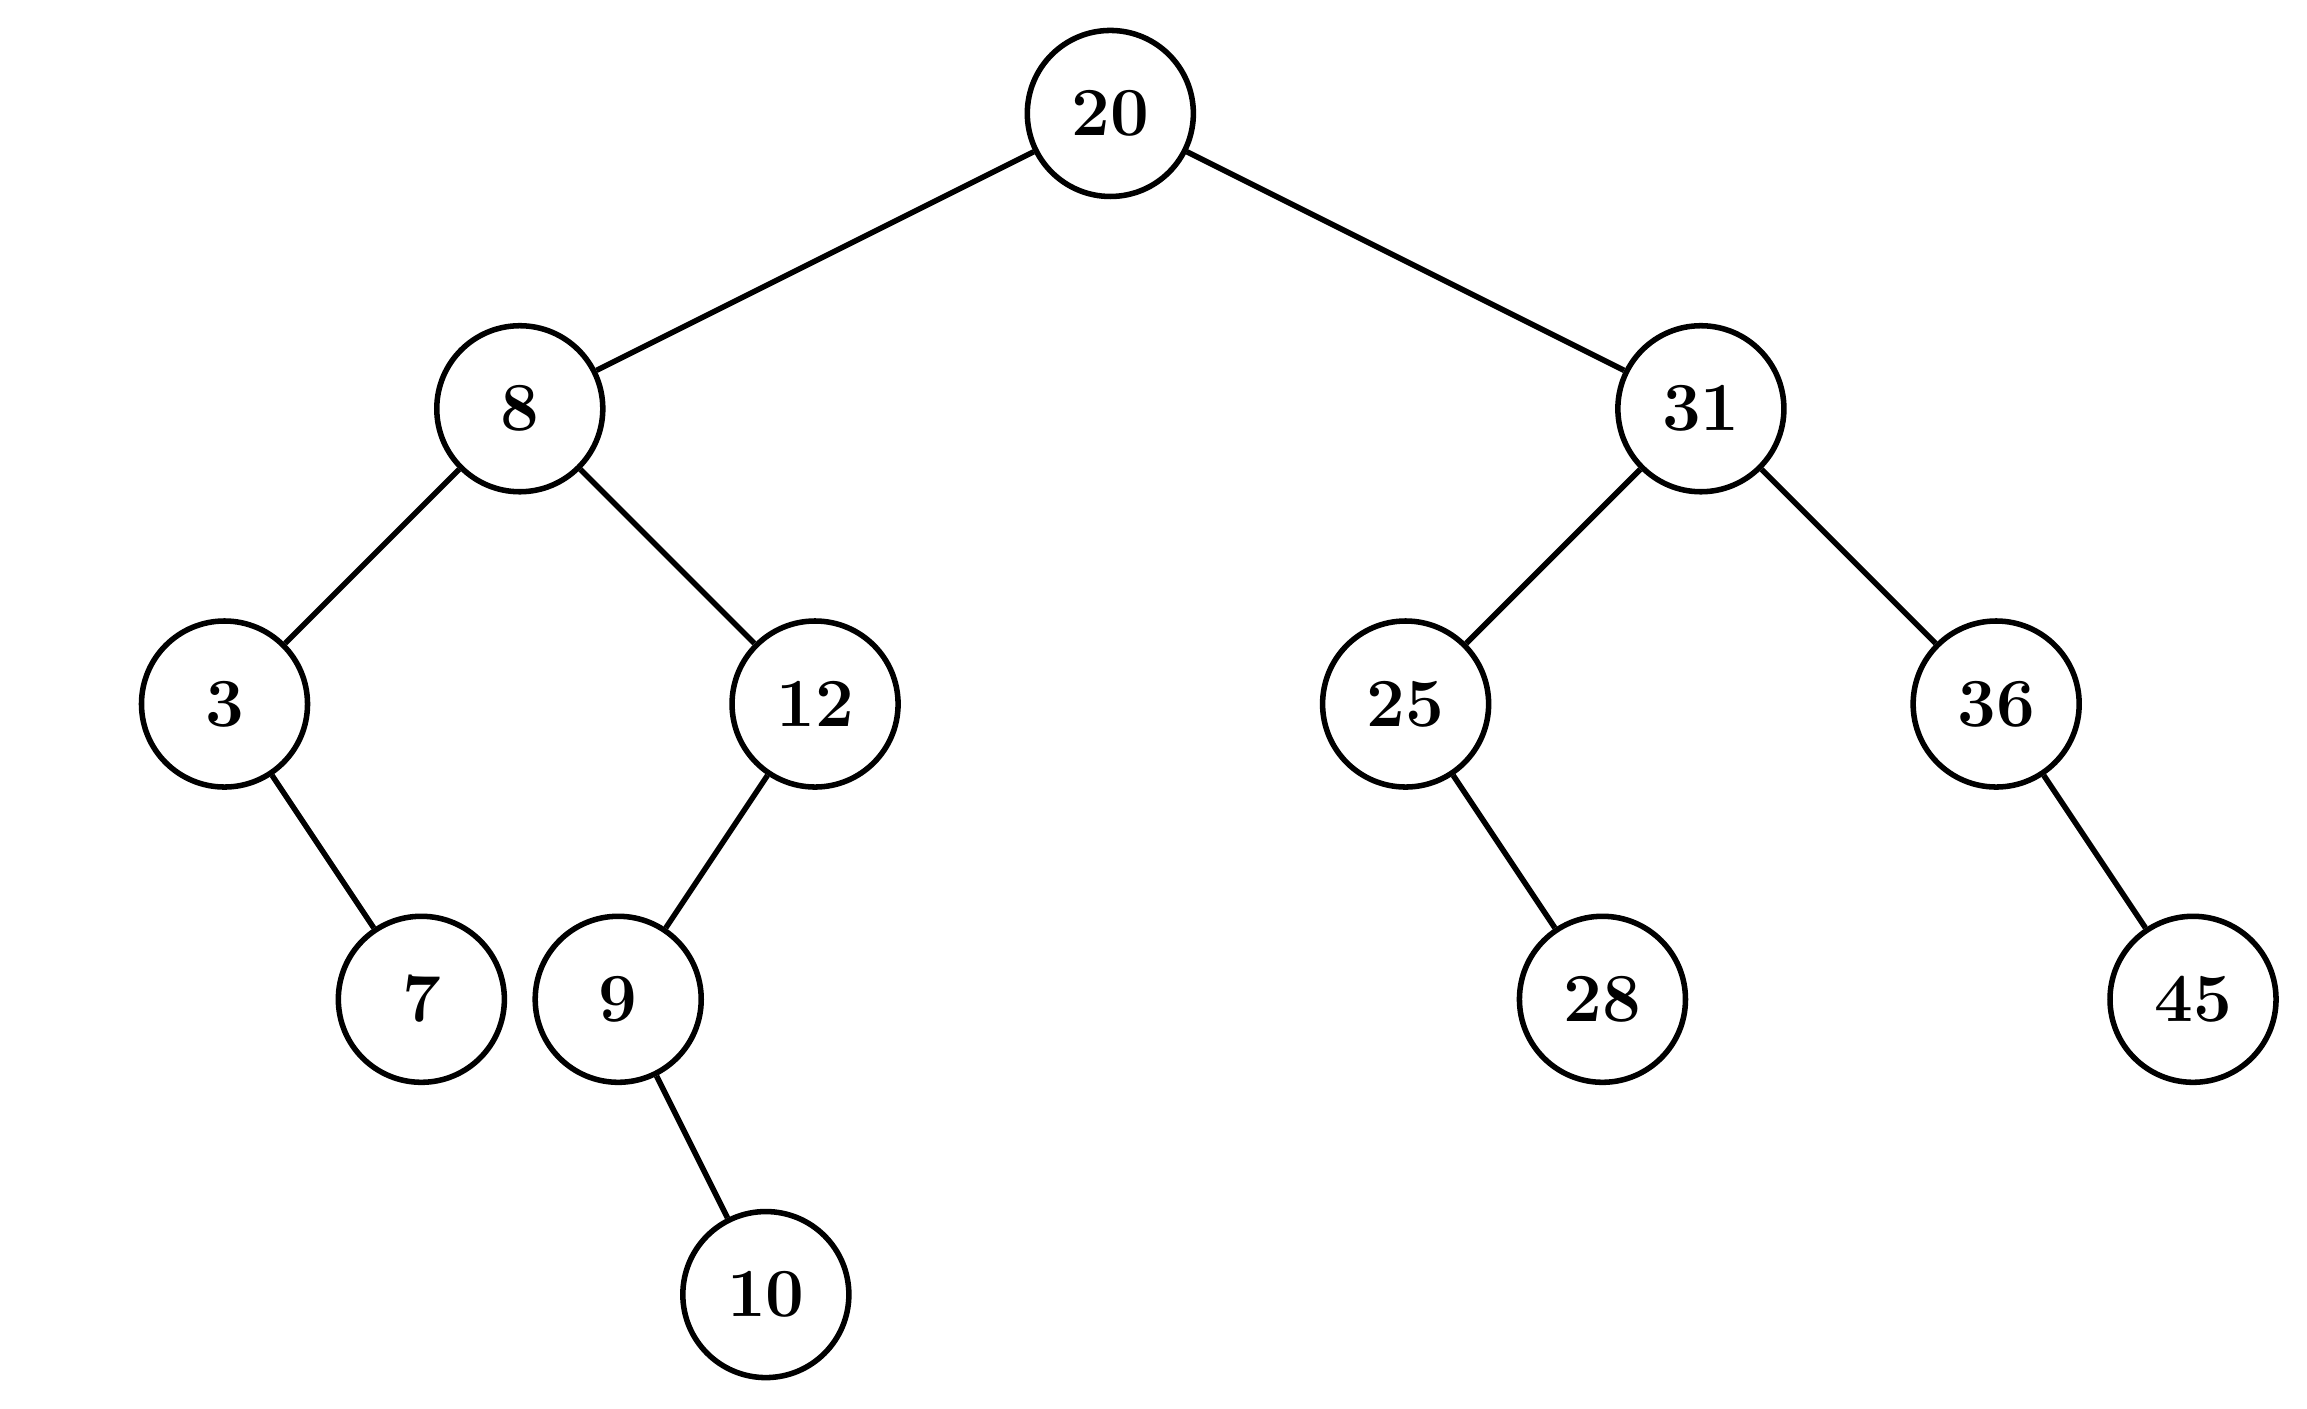
\begin{tikzpicture}[
  scale=2.5,
  every node/.style = {minimum width = 6em, draw, circle, font=\Huge\bf, line width=2pt, scale=1},
  edge from parent/.style={line width=2pt, draw},
  level/.style = {sibling distance = 60mm/#1}
]
  \node {20}
  child {
        node {8}  
        child {
          node {3}
          child {edge from parent[draw = none]}
          child {node {7}}
        }
        child {
          node {12}
          child {
            node {9}
            child {edge from parent[draw = none]}
            child {node {10}}
          }
        child {edge from parent[draw = none]}
        }
      }
  child {
    node {31}
    child {
      node {25}
        child {edge from parent[draw = none]}
      child {node{28}}
    }
    child {
      node {36}
      child {edge from parent[draw = none]}
      child {node{45}}
    }
    };
\end{tikzpicture}
\end{document}

